\part{The backend}\label{part:nstar}


\chapter{Abstract}\label{chap:nstar-abstract}

N* is a \gls{tal} used as a compiler backend (in the same spirit as LLVM, but LLVM is a bit higher level and has concepts like scopes, functions, variables, etc).
Much like any assembly language, files are structured as sections, each containing different types of data.
Each section will be described in details, along with what can be put inside all of them.
They will be studied depending on the target architecture and the target operating system.

\chapter{Target: ELF x86/amd64}\label{chap:elfx86amd64}

The first target of N* is the ELF executable file format, for either x86 or amd64 (amd64 is simply an extension of x86 for 64-bits architectures).

\section{Data section}\label{sec:elf86amd64-data}

The \texttt{data} section in N* is the section where you can bind any value to an address (refered to by a label) that will be used during runtime.
This is most commonly done for static data.

\subsection{Grammar}\label{subsec:elf86amd64-data-grammar}

\begin{figure}[h]
  \centering
  \scalebox{.5}{
    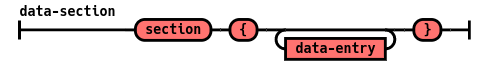
\includegraphics{elf86-amd64-data-grammar-data-section}
  }
\end{figure}
